\documentclass[aspectratio=169,10pt]{beamer}

\usepackage[T1]{fontenc}
\usepackage{booktabs}
\usepackage{tabularx}
\usepackage{graphicx}
\usepackage{tikz}
\usetikzlibrary{arrows.meta,positioning}

\definecolor{primary}{HTML}{1F4E79}
\definecolor{accent}{HTML}{C00000}
\definecolor{softblue}{HTML}{EAF2F8}
\definecolor{softgreen}{HTML}{EAF7EA}
\definecolor{softgray}{HTML}{F4F6F7}
\definecolor{textgray}{HTML}{333333}

\usetheme{default}
\usecolortheme{default}
\setbeamertemplate{navigation symbols}{}
\setbeamercolor{title}{fg=primary}
\setbeamercolor{frametitle}{fg=primary}
\setbeamercolor{normal text}{fg=textgray,bg=white}
\setbeamercolor{block title}{fg=white,bg=primary}
\setbeamercolor{block body}{bg=softgray}
\setbeamertemplate{footline}{%
  \hfill\scriptsize\insertframenumber/\inserttotalframenumber\hspace{0.8em}\vspace{0.5em}
}

\newcommand{\metric}[1]{\textbf{\textcolor{primary}{#1}}}
\newcommand{\risk}[1]{\textbf{\textcolor{accent}{#1}}}

\title{Surrogate-Assisted Online RF Design Optimization}
\subtitle{BCLF results today, spiral inductors next}
\author{Vector RF Optimization}
\date{June 9, 2026}

\begin{document}

\begin{frame}[plain]
  \vspace{0.5cm}
  \titlepage
  \vspace{-0.2cm}
  \begin{center}
    \large
    HFSS-budgeted optimization with a bandpass coupled-line filter testbed,\\
    moving toward template-based spiral inductor design.
  \end{center}
\end{frame}

\begin{frame}{Server--Worker Station Implementation}
  \footnotesize
  \centering
  \resizebox{0.97\linewidth}{!}{%
  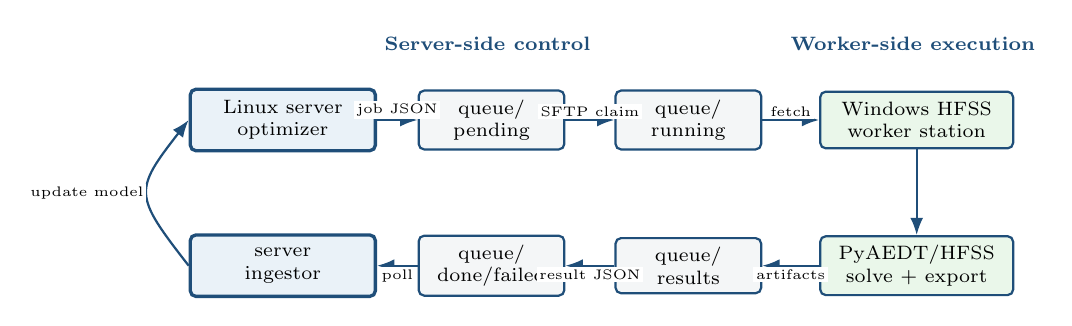
\begin{tikzpicture}[
      station/.style={rounded corners=2pt, draw=primary, fill=softblue,
                      very thick, align=center, minimum width=2.35cm,
                      minimum height=0.78cm, font=\scriptsize},
      queuebox/.style={rounded corners=2pt, draw=primary, fill=softgray,
                       thick, align=center, minimum width=1.85cm,
                       minimum height=0.62cm, font=\scriptsize},
      workerbox/.style={rounded corners=2pt, draw=primary, fill=softgreen,
                        thick, align=center, minimum width=2.45cm,
                        minimum height=0.72cm, font=\scriptsize},
      arrow/.style={-{Latex[length=2.2mm]}, thick, draw=primary},
      note/.style={font=\tiny, fill=white, inner sep=1pt}
    ]
    \node[font=\scriptsize\bfseries, text=primary] at (2.6,2.22) {Server-side control};
    \node[font=\scriptsize\bfseries, text=primary] at (8.0,2.22) {Worker-side execution};

    \node[station] (opt) at (0,1.25) {Linux server\\optimizer};
    \node[queuebox] (pending) at (2.65,1.25) {queue/\\pending};
    \node[queuebox] (running) at (5.15,1.25) {queue/\\running};
    \node[workerbox] (worker) at (8.05,1.25) {Windows HFSS\\worker station};

    \node[station] (ingest) at (0,-0.60) {server\\ingestor};
    \node[queuebox] (done) at (2.65,-0.60) {queue/\\done/failed};
    \node[queuebox] (results) at (5.15,-0.60) {queue/\\results};
    \node[workerbox] (hfss) at (8.05,-0.60) {PyAEDT/HFSS\\solve + export};

    \draw[arrow] (opt) -- node[note,above]{job JSON} (pending);
    \draw[arrow] (pending) -- node[note,above]{SFTP claim} (running);
    \draw[arrow] (running) -- node[note,above]{fetch} (worker);
    \draw[arrow] (worker) -- (hfss);
    \draw[arrow] (hfss) -- node[note,below]{artifacts} (results);
    \draw[arrow] (results) -- node[note,below]{result JSON} (done);
    \draw[arrow] (done) -- node[note,below]{poll} (ingest);
    \draw[arrow] (ingest.west) .. controls +(-0.70,0.90) and +(-0.70,-0.90) ..
      node[note,left]{update model} (opt.west);
  \end{tikzpicture}
  }

  \vspace{0.22cm}
  \begin{columns}[T,onlytextwidth]
    \begin{column}{0.48\textwidth}
      \begin{block}{Boundary}
        Server selects candidates and ingests results; it never calls HFSS.
      \end{block}
    \end{column}
    \begin{column}{0.48\textwidth}
      \begin{block}{Worker contract}
        One job JSON in; one done/failed JSON plus Touchstone artifacts out.
      \end{block}
    \end{column}
  \end{columns}
\end{frame}

\begin{frame}{BCLF Problem Setup}
  \footnotesize
  \begin{columns}[T,onlytextwidth]
    \begin{column}{0.47\textwidth}
      \begin{block}{Design vector}
        \[
          x = [L,L1,L2,W,W1,W2,S1,S2]
        \]
        \vspace{-0.25cm}
        \begin{itemize}
          \item Eight geometry variables in mm
          \item Bounds from the shared BCLF config
          \item Candidate geometry snapped to \metric{0.01 mm}
          \item Queue-backed HFSS or cache lookup
        \end{itemize}
      \end{block}
      \vspace{0.15cm}
      \begin{block}{Optimization convention}
        Minimize one scalar objective derived from simulated \metric{S11} and
        \metric{S21}. Lower best-so-far is better.
      \end{block}
    \end{column}
    \begin{column}{0.50\textwidth}
      \scriptsize
      \begin{tabularx}{\linewidth}{@{}lX@{}}
        \toprule
        Item & Current BCLF target \\
        \midrule
        Passband & $[4.8, 5.4]$ GHz \\
        Lower stopband & $[3.6, 4.4]$ GHz \\
        Upper stopband & $[5.8, 8.7]$ GHz \\
        Passband S21 & worst value $\ge -5.0$ dB \\
        Passband S11 & worst value $\le -7.0$ dB \\
        Stopband S21 & worst value $\le -15.0$ dB \\
        Frequency grid & 3.5--8.713 GHz, 401 points \\
        \bottomrule
      \end{tabularx}
      \vspace{0.25cm}
      \begin{block}{Why this is hard}
        Each new candidate may trigger an HFSS solve, so method comparisons
        must count trials, seeds, cache hits, and initialization policy.
      \end{block}
    \end{column}
  \end{columns}
\end{frame}

\begin{frame}{Shared Online Optimization Backbone}
  \centering
  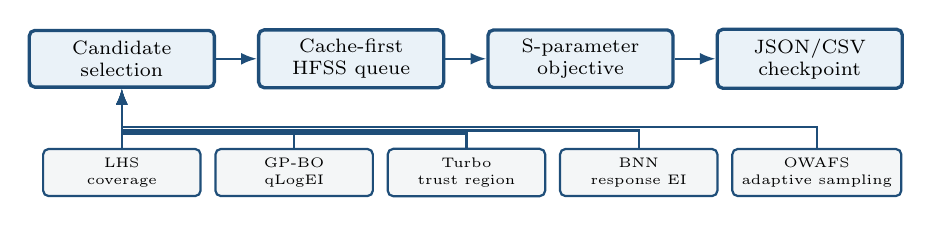
\begin{tikzpicture}[
      node distance=0.52cm,
      box/.style={rounded corners=2pt, draw=primary, fill=softblue, very thick,
                  align=center, minimum width=2.35cm, minimum height=0.72cm,
                  font=\scriptsize},
      smallbox/.style={rounded corners=2pt, draw=primary, fill=softgray, thick,
                  align=center, minimum width=2.0cm, minimum height=0.55cm,
                  font=\tiny},
      arrow/.style={-{Latex[length=2mm]}, thick, draw=primary}
    ]
    \node[box] (select) {Candidate\\selection};
    \node[box, right=of select] (sim) {Cache-first\\HFSS queue};
    \node[box, right=of sim] (score) {S-parameter\\objective};
    \node[box, right=of score] (save) {JSON/CSV\\checkpoint};
    \draw[arrow] (select) -- (sim);
    \draw[arrow] (sim) -- (score);
    \draw[arrow] (score) -- (save);

    \node[smallbox, below=0.75cm of select] (lhs) {LHS\\coverage};
    \node[smallbox, right=0.16cm of lhs] (bo) {GP-BO\\qLogEI};
    \node[smallbox, right=0.16cm of bo] (turbo) {Turbo\\trust region};
    \node[smallbox, right=0.16cm of turbo] (bnn) {BNN\\response EI};
    \node[smallbox, right=0.16cm of bnn] (owafs) {OWAFS\\adaptive sampling};
    \draw[arrow] (lhs.north) -- ++(0,0.26) -| (select.south);
    \draw[arrow] (bo.north) -- ++(0,0.22) -| (select.south);
    \draw[arrow] (turbo.north) -- ++(0,0.18) -| (select.south);
    \draw[arrow] (bnn.north) -- ++(0,0.22) -| (select.south);
    \draw[arrow] (owafs.north) -- ++(0,0.26) -| (select.south);
  \end{tikzpicture}

  \vspace{0.35cm}
  \scriptsize
  \begin{tabularx}{0.96\linewidth}{@{}lX@{}}
    \toprule
    Method & Role in the current evidence chain \\
    \midrule
    LHS & Strong coverage baseline; surprisingly competitive under 80-trial budgets. \\
    GP-BO / Turbo & Classical surrogate baselines; now refactored to continuous acquisition plus snapping. \\
    BNN & Learns response curves, then ranks sampled candidates through the same objective. \\
    OWAFS & Diagnostic adaptive sampler from a 15-point previous-LHS warmup. \\
    \bottomrule
  \end{tabularx}
\end{frame}

\begin{frame}{GPBO, BNN, and OWAFS Differ}
  \footnotesize
  \begin{columns}[T,onlytextwidth]
    \begin{column}{0.31\textwidth}
      \begin{block}{GPBO}
        \scriptsize
        \[
          \alpha_{GP}(x)=\mathrm{qLogEI}(\mu_t,\sigma_t)
        \]
        \[
          x_{t+1}=\mathrm{snap}_{0.01}
          \left(\arg\max_x \alpha_{GP}(x)\right)
        \]
        Scalar GP models the completed objective values.
      \end{block}
    \end{column}
    \begin{column}{0.31\textwidth}
      \begin{block}{BNN}
        \scriptsize
        \[
          \hat y(x)=g(\hat S_{11}(x,f),\hat S_{21}(x,f))
        \]
        \[
          x_{t+1}=\arg\max_{x\in\mathcal B_t}
          \mathrm{EI}_{BNN}(x)
        \]
        $\mathcal B_t$ is freshly sampled from bounds.
      \end{block}
    \end{column}
    \begin{column}{0.31\textwidth}
      \begin{block}{OWAFS}
        \scriptsize
        \[
          a(f)=w(f)\,\frac{R(f)+U(f)}{2}
        \]
        \[
          R=\rho(r_{VF}),\quad U=\rho(u_{BNN})
        \]
        $\rho$: rank-normalize to $[0,1]$ after warmup.
      \end{block}
    \end{column}
  \end{columns}

  \vspace{0.28cm}
  \begin{columns}[T,onlytextwidth]
    \begin{column}{0.48\textwidth}
      \begin{block}{Common ground}
        \begin{itemize}
          \item Same BCLF objective and simulator adapter.
          \item Same artifact style: history, CSV, checkpoint.
          \item Lower best-so-far objective is better.
        \end{itemize}
      \end{block}
    \end{column}
    \begin{column}{0.48\textwidth}
      \begin{block}{Important boundary}
        OWAFS and current BNN/BO runs differ in initialization policy, so the
        current deck reports evidence rather than a final method ranking.
      \end{block}
    \end{column}
  \end{columns}
\end{frame}

\begin{frame}{Current Online Results}
  \begin{columns}[T,onlytextwidth]
    \begin{column}{0.57\textwidth}
      \includegraphics[width=\linewidth]{figures/owafs_vs_bo_lhs_bnn_best_so_far_objective.png}
    \end{column}
    \begin{column}{0.41\textwidth}
      \scriptsize
      \begin{tabular}{@{}lrr@{}}
        \toprule
        Method & Seeds & Median best \\
        \midrule
        BO & 5 & -14.657 \\
        LHS & 5 & \textbf{-19.162} \\
        Turbo & 5 & -19.161 \\
        BNN & 5 & -17.342 \\
        OWAFS & 5 & -17.413 \\
        \bottomrule
      \end{tabular}

      \vspace{0.35cm}
      \begin{block}{Current claim boundary}
        \begin{itemize}
          \item BNN beats BO by median final best.
          \item LHS/Turbo remain stronger references.
          \item OWAFS improves its warmup, but initialization differs.
          \item No strict superiority claim yet.
        \end{itemize}
      \end{block}
    \end{column}
  \end{columns}
\end{frame}

\begin{frame}{Recent BO/BNN Diagnostic}
  \centering
  \includegraphics[height=0.65\textheight]{figures/bo_continuous_ninit10_seed0_vs_bnn_online_general_objective.png}

  \vspace{0.1cm}
  \begin{block}{Status at deck generation}
    \scriptsize
    \begin{itemize}
      \item Continuous BO: seed 0, $n_{\mathrm{init}}=10$, \metric{70/80} trials complete, best \metric{-16.759}.
      \item BNN online-general: seed 0 complete, $n_{\mathrm{init}}=30$, best \metric{-24.999}; not matched initialization.
    \end{itemize}
  \end{block}
\end{frame}

\begin{frame}{Roadmap: Spiral Inductor Extension}
  \begin{columns}[T,onlytextwidth]
    \begin{column}{0.47\textwidth}
      \begin{block}{Template already planned}
        \begin{itemize}
          \item Square spiral, fixed 3 turns
          \item Variables: \metric{Din, W, S, H}
          \item Two-port lumped excitation
          \item Export `.s2p` over 0.1--30 GHz
          \item Extract $L(5\mathrm{GHz})$, $Q(5\mathrm{GHz})$, SRF
        \end{itemize}
      \end{block}
    \end{column}
    \begin{column}{0.50\textwidth}
      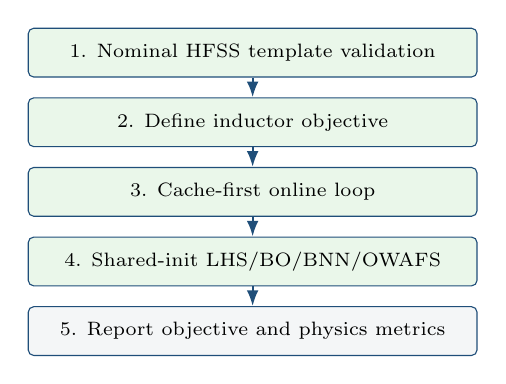
\begin{tikzpicture}[
          roadmapstep/.style={rounded corners=2pt, draw=primary, fill=softgreen,
                       minimum width=5.7cm, minimum height=0.62cm,
                       align=left, font=\scriptsize},
          arrow/.style={-{Latex[length=2mm]}, thick, draw=primary}
        ]
        \node[roadmapstep] (a) {1. Nominal HFSS template validation};
        \node[roadmapstep, below=0.25cm of a] (b) {2. Define inductor objective};
        \node[roadmapstep, below=0.25cm of b] (c) {3. Cache-first online loop};
        \node[roadmapstep, below=0.25cm of c] (d) {4. Shared-init LHS/BO/BNN/OWAFS};
        \node[roadmapstep, below=0.25cm of d, fill=softgray] (e) {5. Report objective and physics metrics};
        \draw[arrow] (a) -- (b);
        \draw[arrow] (b) -- (c);
        \draw[arrow] (c) -- (d);
        \draw[arrow] (d) -- (e);
      \end{tikzpicture}
    \end{column}
  \end{columns}

  \vspace{0.2cm}
  \begin{block}{Near-term risks to retire}
    Template sanity, physically meaningful objectives, fair seed sharing, and
    response-surrogate transfer from BCLF to inductor metrics.
  \end{block}
\end{frame}

\end{document}
